\begin{wrapfigure}[18]{r}[0pt]{38mm}
	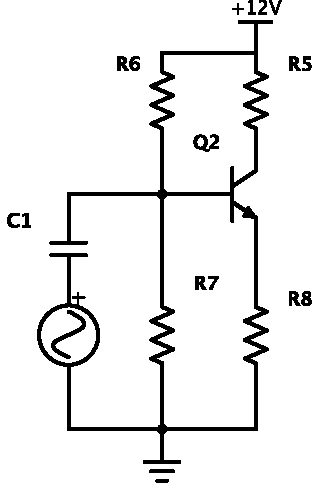
\includegraphics[width=38mm]{cc2.pdf}
	\caption{Amplificatore ad emettitore comune.}
	\label{fig:cc2}
\end{wrapfigure}

\section{Amplificatore ad emettitore comune}

Riportiamo in Fig. \ref{fig:cc2} lo schema del circuito utilizzato per questa seconda parte dell'esperienza.
Anche in questo caso abbiamo dovuto dimensionare le resistenze del partitore e inoltre anche la capacità $C_1$.
Avendo scelto come $R_E=(498.4\pm0.1)\,\si{\ohm}$ e volendo una corrente di quiescenza di $\approx \SI{1}{\milli\ampere}$ abbiamo stimato $V_B=\SI{1.1}{\volt}$.
Possiamo ora, attraverso Eq. (\ref{partitore}), calcolare i valori di $R_1$ e $R_2$.
Avendo anche in questo caso scelto $R_1=(100.03\pm0.2)\,\si{\kilo\ohm}$ abbiamo utilizzato una $R_2=(12.16\pm0.01)\,\si{\kilo\ohm}$.
Come segnale in ingresso è stata usata una forma d'onda sinusoidale a frequenza di $\SI{1}{\kilo\hertz}$.
Per la struttura del circuito risulta semplice impostare il calcolo di $C_1$.
Infatti il condensatore è caricato dal parallelo delle resistenze del partitore e dall'impedenza in ingresso del transistor, $Z_in=\beta R_E$.
Inoltre, esso fa parte di una sorta di filtro passa alto.
Basterà dunque utilizzare dei valori di capacità adeguati in modo da avere una frequenza di taglio minore di $\SI{1}{\kilo\hertz}$.
Riportiamo l'equazione utilizzata per il calcolo di $C_1$

\begin{equation}
C_1>>\frac{1}{2 \pi \cdot R_1 // R_2//\beta R_E}
\end{equation}

Inserendo i nostri valori, otteniamo $C_1>>\SI{15}{\nano\farad}$.
È stato dunque scelto di usare un uno dei primi condensatori trovati sul tavolo con capacità $C_1=(0.982\pm0.005)\,\si{\micro\farad}$.
Per la nostra esperienza era richiesto un guadagno in tensione pari a $G=-10$.
Ricordando che $G\doteqdot - \frac{R_C}{R_E}$ è stata utilizzata una $R_C=(4.969\pm0.001)\,\si{\kilo\ohm}$. 

Stimati tutti i valori delle componenti circuitali, abbiamo montato il circuito vero e riportato a schermo dell'oscilloscopio sia segnale in ingresso che in uscita.
Nel seguente grafico sono riportati i dati dell'oscilloscopio.

\begin{figure}[H]
\centering
	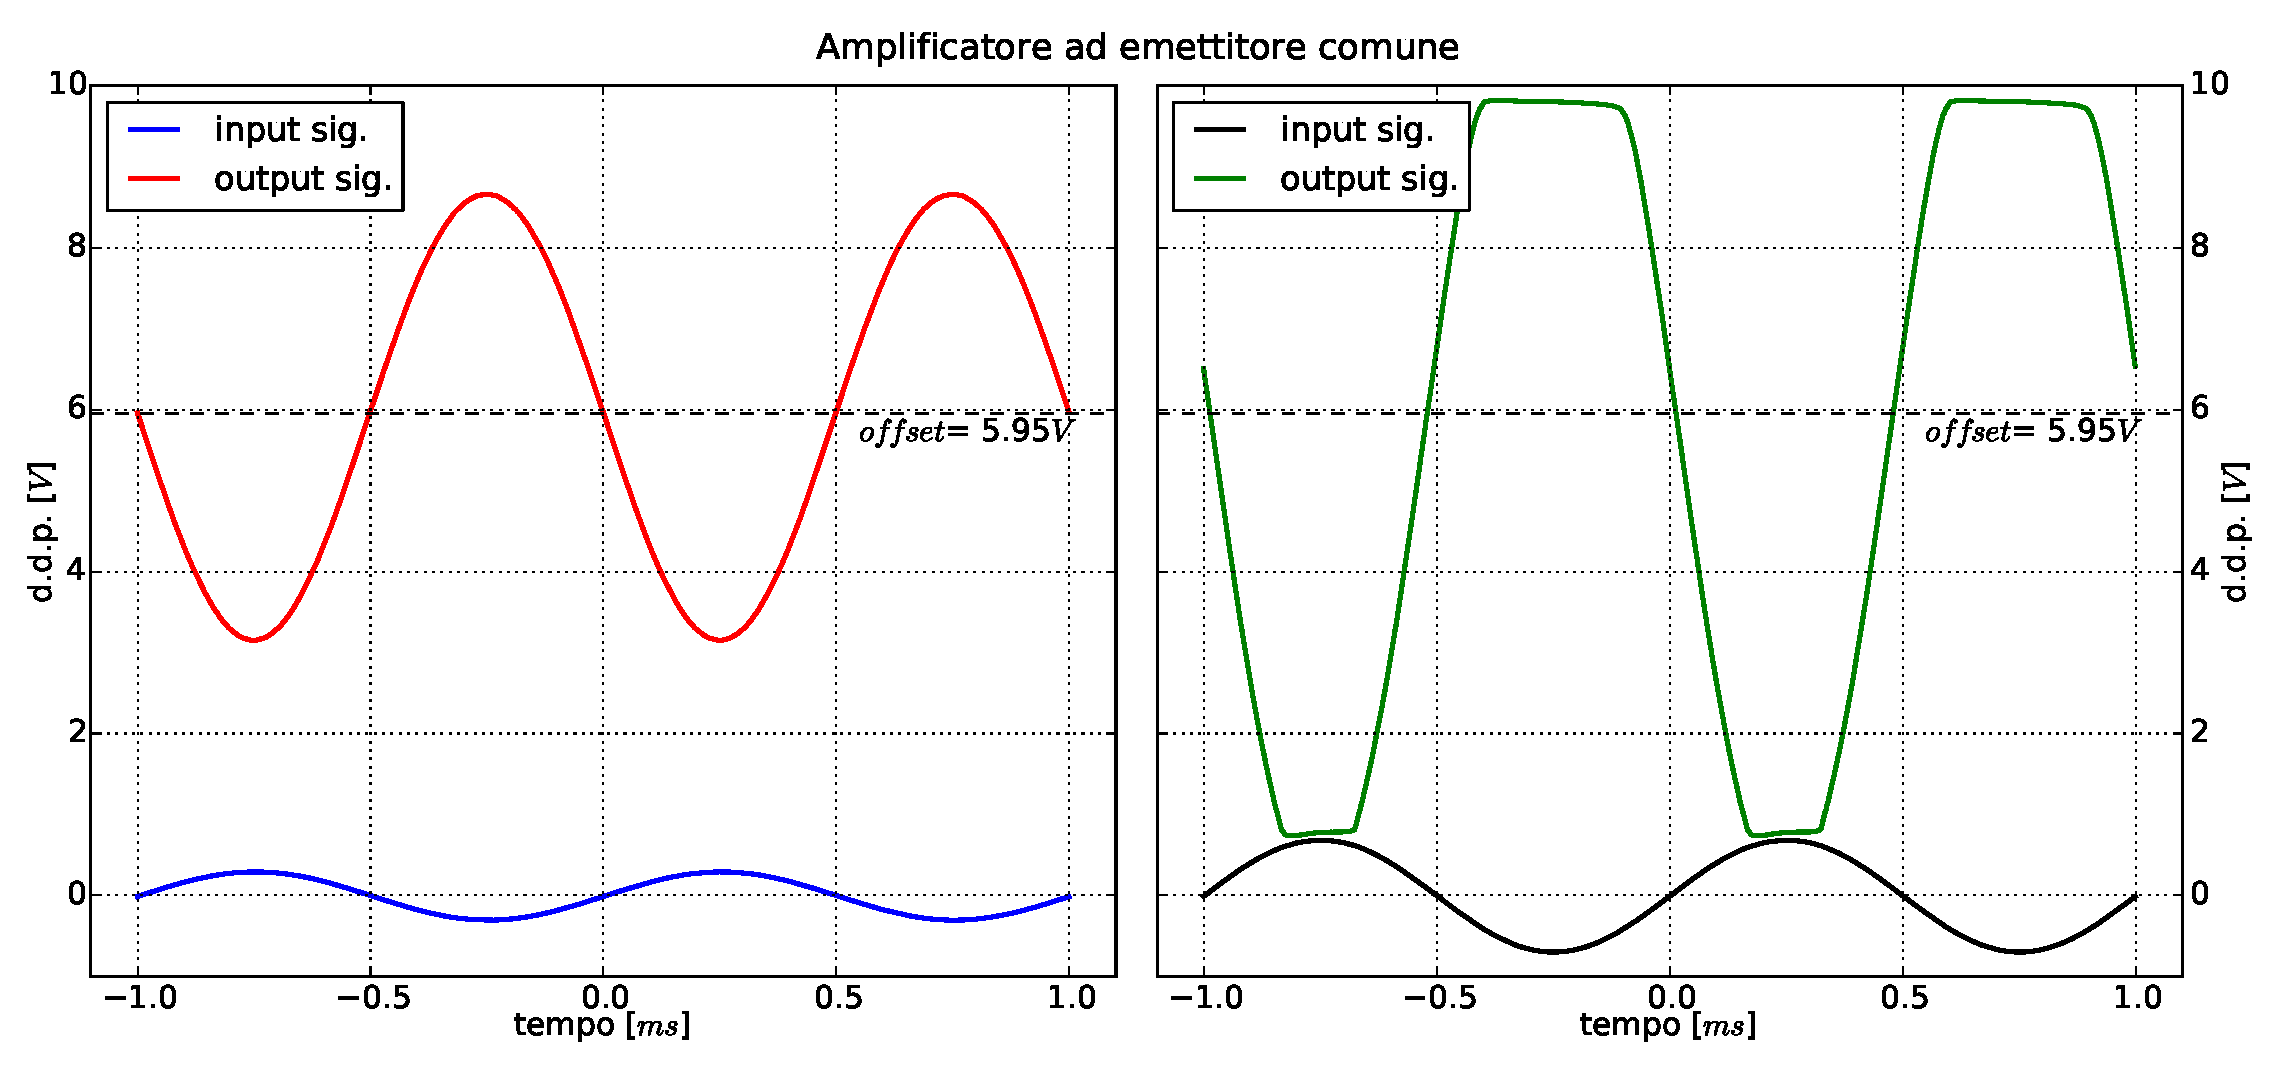
\includegraphics[scale=0.45]{amp.pdf}
	\caption{Amplificatore ad emettitore comune. Nel grafico a sinistra è riportato il comportamento dell'amplificatore nella zona ottimale, mentre nella zona a destra è riportato l'andamento del segnale in uscite nelle condizioni di ``\emph{clipping}''. Come vediamo tale fenomeno si realizza per tensioni oltre $\approx 10V$ (tensione $V_{CC}$) e inferiori a $\approx 0.6V$ (tensione minima $V_{BE}$). }
	\label{fig:amp}
\end{figure}

Come vediamo immediatamente, il segnale in uscita è sfasato di $\pi$.
Proprio per questo motivo nella formula del guadagno compare quel segno meno.
Dai dati sperimentali è stato possibile stimare il valore di guadagno effettivo, utilizzando la tensione picco-picco:

$$G_{exp}=-(9.2 \pm 0.1)$$

Per ovviare al problema dell'$offset$ del segnale in uscita potremmo inserire un capacitore. Così facendo elimineremmo infatti la componente continua del segnale. 

\begin{wrapfigure}[18]{r}[0pt]{36mm}
	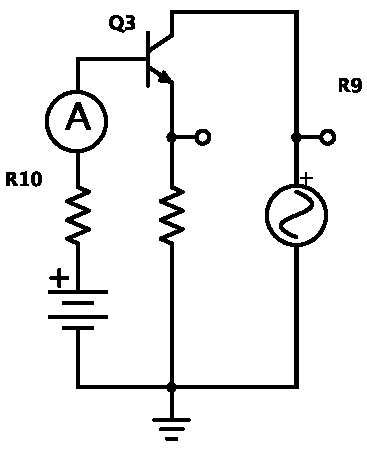
\includegraphics[width=36mm]{cc3.pdf}
	\caption{Sorgente di corrente costante.}
	\label{fig:cc3}
\end{wrapfigure}

\section{Caratteristica di uscita}

In questa ultima parte dell'esperienza abbiamo cercato di analizzare la caratteristica di uscita del transistor.
Per fare ciò abbiamo montato il circuito in Fig. \ref{fig:cc3}.

Alimentandolo con un'onda sinusoidale di frequenza $\SI{1}{\kilo\hertz}$, con tensione picco-picco $V_{pp} = \SI{10}{\volt}$ e offset di $+\SI{5}{\volt} \, DC$ e impostando l'oscilloscopio in configurazione XY, possiamo ottenere la caratteristica di uscita per diverse correnti di base (impostate cambiando la $V_B$).

\begin{figure}[h]
\centering
	\caption{Caratteristica di uscita del transistor}
	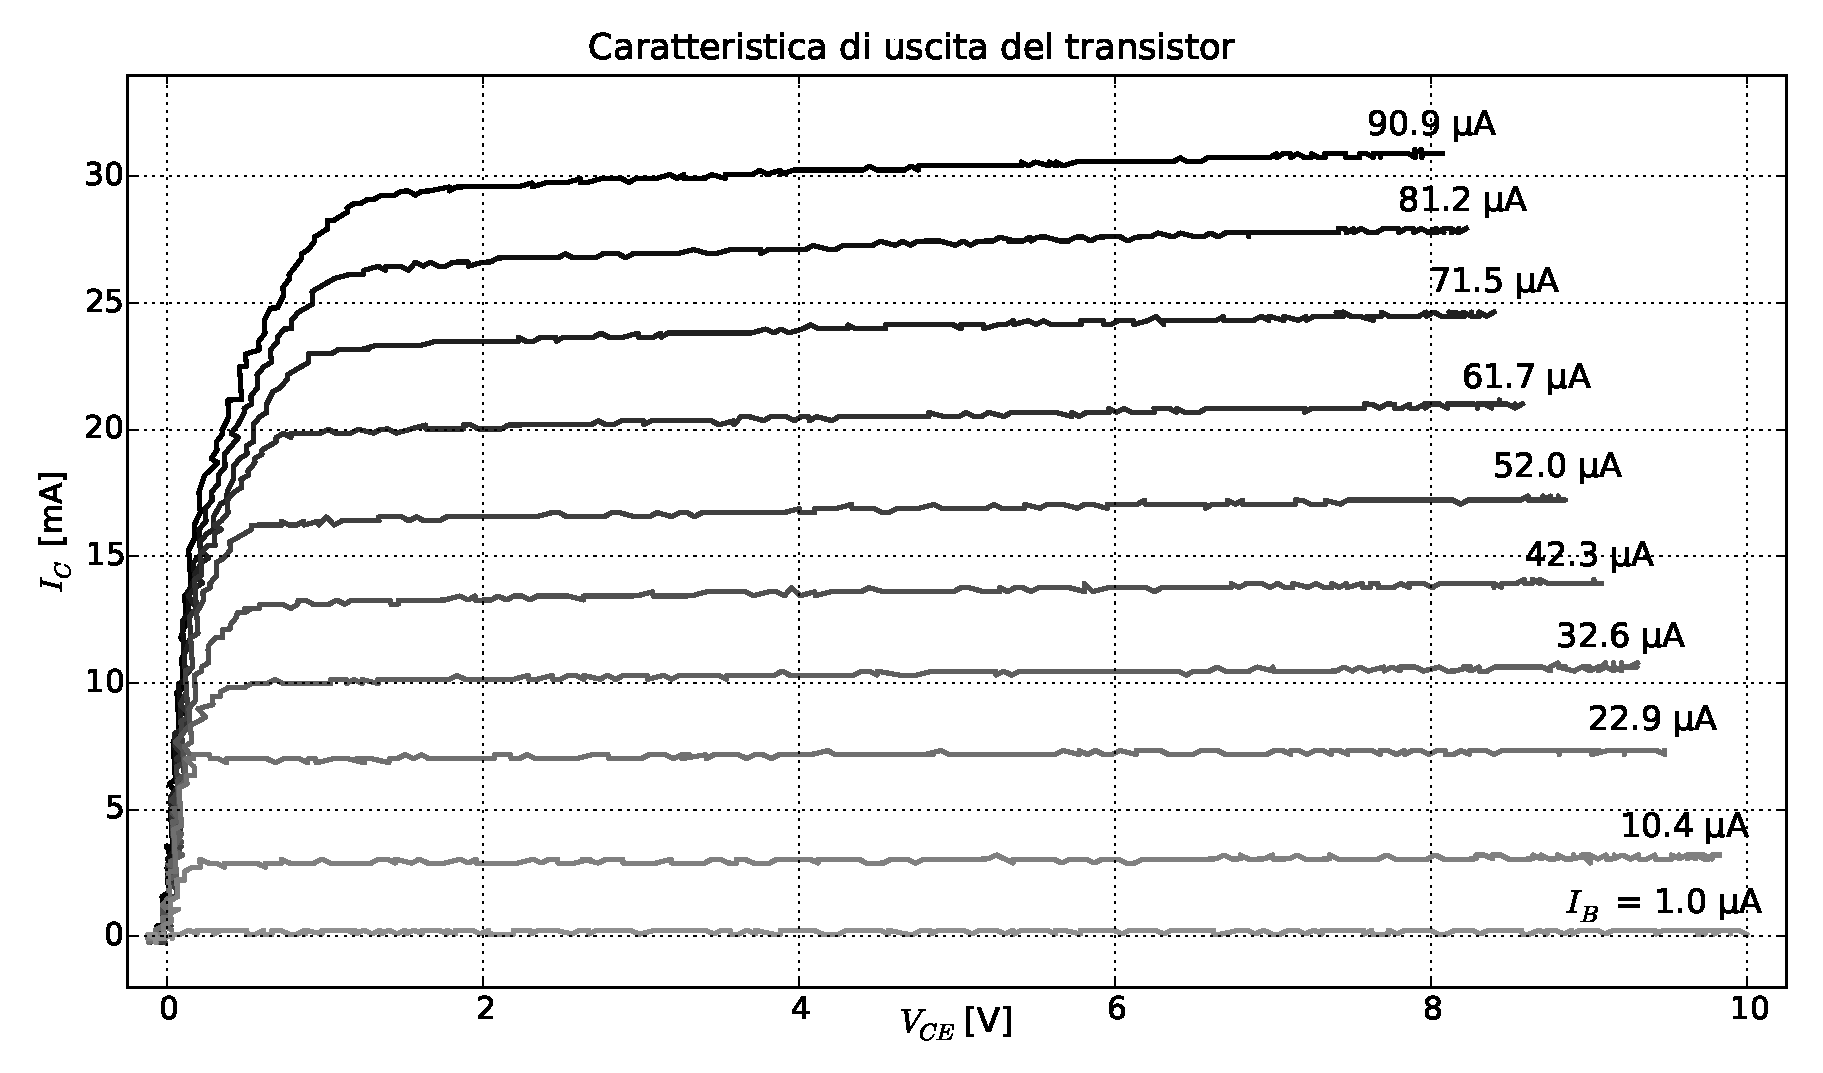
\includegraphics[scale=0.45]{xy.pdf}
	\label{fig:xy}
\end{figure}